% =============================================================================
%  Beamer — "What Happens Next?" — focus modèles
%  Étienne Chevrolat, CSC_43M04_EP
% =============================================================================
\documentclass[10pt,aspectratio=169]{beamer}

\usetheme{Boadilla}
\usecolortheme{seahorse}
\setbeamertemplate{navigation symbols}{}

\usepackage[utf8]{inputenc}
\usepackage[T1]{fontenc}
\usepackage{amsmath,amssymb}
\usepackage{booktabs}
\usepackage{array}
\usepackage{tikz}
\usetikzlibrary{arrows.meta, positioning, fit, calc, backgrounds, shapes.geometric, decorations.pathreplacing}

\definecolor{accent}{HTML}{1f6feb}
\definecolor{good}{HTML}{1a7f37}
\definecolor{warn}{HTML}{9a6700}
\definecolor{bad}{HTML}{c1272d}
\definecolor{bgblock}{HTML}{eaf2fb}
\definecolor{bgconv}{HTML}{fff4d6}
\definecolor{bgtrans}{HTML}{f4e4ff}
\definecolor{bgmae}{HTML}{ffe0d0}
\definecolor{gridgray}{HTML}{cccccc}
\setbeamercolor{alerted text}{fg=accent}

% Styles TikZ pour diagrammes académiques (taille FIXE → pas de superposition)
\tikzset{
  blkconv/.style  = {draw, rounded corners=2pt, fill=bgconv,
                     minimum width=20mm, minimum height=11mm,
                     font=\scriptsize\ttfamily, align=center, inner sep=2pt},
  blktrans/.style = {draw, rounded corners=2pt, fill=bgtrans,
                     minimum width=20mm, minimum height=11mm,
                     font=\scriptsize\ttfamily, align=center, inner sep=2pt},
  blkmisc/.style  = {draw, rounded corners=2pt, fill=bgblock,
                     minimum width=20mm, minimum height=11mm,
                     font=\scriptsize\ttfamily, align=center, inner sep=2pt},
  blkmae/.style   = {draw, rounded corners=2pt, fill=bgmae,
                     minimum width=20mm, minimum height=11mm,
                     font=\scriptsize\ttfamily, align=center, inner sep=2pt},
  blkio/.style    = {draw=accent, very thick, rounded corners=2pt,
                     minimum width=18mm, minimum height=10mm,
                     font=\scriptsize\bfseries, align=center, inner sep=2pt},
  flow/.style     = {-{Latex[length=1.8mm]}, thick},
  dimlbl/.style   = {font=\tiny\itshape, fill=white, inner sep=1pt},
}

\newcommand{\hl}[1]{\textcolor{accent}{\textbf{#1}}}
\newcommand{\good}[1]{\textcolor{good}{\textbf{#1}}}

\title[What Happens Next?]{What Happens Next? --- Synthèse des modèles}
\subtitle{Classification vidéo, 33 classes, $T=4$ frames}
\author{Étienne Chevrolat}
\institute{CSC\_43M04\_EP}
\date{\today}

\begin{document}

\maketitle

% =============================================================================
\begin{frame}{Les différentes architectures testées}
  \medskip
  \begin{itemize}
    \item \texttt{model4\_A} : idée initiale \textbf{CNN 2D + temporal attention}.
    \item \texttt{model5\_A} / \texttt{model5\_B} : \textbf{R(2+1)D + transformer} ; \texttt{5\_B} avec TSM + 196 tokens spatio-temporels.
    \item \texttt{videomae\_v2} + \texttt{model7\_A} : pretrain self-supervisé (94M params) puis finetune ViT-B avec LLDR.
  \end{itemize}
\end{frame}

% =============================================================================
\section{Vue d'ensemble}
% =============================================================================

\begin{frame}{Récapitulatif des meilleurs runs}
  \footnotesize
  \begin{tabular}{l l r r r r}
    \toprule
    \textbf{Ckpt} & \textbf{Archi} & \textbf{Params} & \textbf{top-1} & \textbf{top-5} & \textbf{lat. ms/clip} \\
    \midrule
    \texttt{best\_model.pt}              & model1.2\_A          & 12.9M & 0.244 & 0.548 & 1.3 \\
    \texttt{best\_model\_v2.pt}          & model2\_A            & 17.8M & 0.229 & 0.535 & 1.6 \\
    \texttt{best\_model\_v6\_5.pt}       & model5\_B            & 39.8M & 0.357 & 0.677 & 4.2 \\
    \texttt{best\_model\_v6\_8.pt}       & model5\_B            & 39.8M & 0.403 & 0.718 & 4.2 \\
    \texttt{best\_model\_v6\_10.pt}      & model5\_B            & 39.8M & 0.405 & 0.715 & 4.2 \\
    \alert{\texttt{best\_model\_v6\_12.pt}} & \alert{model5\_B} & \alert{39.8M} & \alert{\good{0.406}} & \alert{\good{0.719}} & 4.2 \\
    \texttt{best\_model\_v6\_101.pt}     & model5\_B            & 42.9M & 0.391 & 0.701 & 4.3 \\
    \texttt{best\_model\_v7\_lldr\_v2}   & model7\_A            & 86.3M & 0.401 & 0.715 & 9.2 \\
    \alert{\texttt{best\_model\_v7\_lldr\_diverse}} & \alert{model7\_A} & \alert{86.3M} & \alert{\good{0.409}} & \alert{\good{0.736}} & \alert{9.2} \\
    \bottomrule
  \end{tabular}
\end{frame}

\begin{frame}{Précision vs taille / latence}
  \centering
  \begin{tikzpicture}[x=0.0011cm, y=22cm]
    \draw[->] (0,0.20) -- (10500,0.20) node[below right, font=\scriptsize] {params (M$\to$)};
    \draw[->] (0,0.20) -- (0,0.48) node[above left, font=\scriptsize] {real val top-1};
    \foreach \y in {0.20, 0.25, 0.30, 0.35, 0.40, 0.45} {
      \draw[gridgray, very thin] (0,\y) -- (10500,\y);
      \node[left, font=\tiny] at (0,\y) {\y};
    }
    \foreach \x in {0, 20, 40, 60, 80, 100} {
      \draw[gridgray, very thin] (\x*100, 0.20) -- (\x*100, 0.46);
      \node[below, font=\tiny] at (\x*100, 0.20) {\x};
    }
    \foreach \xc/\yc/\lab/\col in {%
      1290/0.244/m1.2\_A/warn,
      1780/0.229/m2\_A/warn,
      3980/0.357/m5\_B v6\_5/accent,
      3980/0.405/m5\_B v6\_10/accent,
      3980/0.406/m5\_B v6\_12/good,
      8626/0.401/m7 lldr v2/accent,
      8626/0.409/m7 lldr div/good%
    } {
      \filldraw[fill=\col, draw=black, fill opacity=0.6] (\xc, \yc) circle (0.012);
      \node[right=2pt, font=\tiny] at (\xc, \yc) {\texttt{\lab}};
    }
    \draw[good, dashed, thick] (3980,0.406) -- (8626, 0.409);
    \node[good, font=\tiny] at (6500, 0.42) {Pareto-optimal};
  \end{tikzpicture}

  \footnotesize \texttt{model5\_B} reste \hl{2$\times$ plus petit et 2$\times$ plus rapide} que \texttt{model7\_A} pour une accuracy quasi-équivalente.
\end{frame}

% =============================================================================
\section{model4\_A : l'idée initiale}
% =============================================================================

\begin{frame}{model4\_A --- CNN 2D + temporal attention}
  \textbf{Idée.} Un CNN 2D produit \emph{un vecteur par frame} ; un mini-transformer agrège les $T{+}1$ tokens.

  \medskip
  \centering
  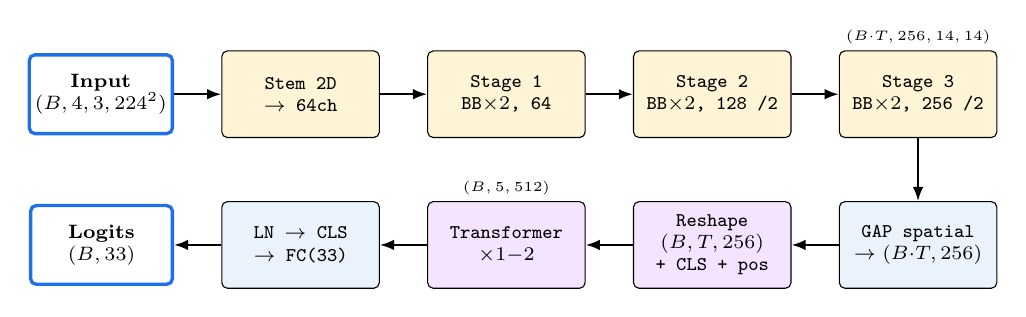
\begin{tikzpicture}[node distance=8mm and 6mm]
    % Row 1 : spatial backbone (gauche -> droite)
    \node[blkio]                                  (in)   {Input\\$(B,4,3,224^2)$};
    \node[blkconv, right=of in]                   (stem) {Stem 2D\\$\to$ 64ch};
    \node[blkconv, right=of stem]                 (s1)   {Stage 1\\BB$\times 2$, 64};
    \node[blkconv, right=of s1]                   (s2)   {Stage 2\\BB$\times 2$, 128 /2};
    \node[blkconv, right=of s2]                   (s3)   {Stage 3\\BB$\times 2$, 256 /2};
    % Row 2 : temporal head (droite -> gauche, sous Row 1)
    \node[blkmisc, below=of s3]                   (gap)  {GAP spatial\\$\to (B{\cdot}T, 256)$};
    \node[blktrans, left=of gap]                  (tok)  {Reshape\\$(B,T,256)$\\+ CLS + pos};
    \node[blktrans, left=of tok]                  (tx)   {Transformer\\$\times 1{-}2$};
    \node[blkmisc, left=of tx]                    (head) {LN $\to$ CLS\\$\to$ FC(33)};
    \node[blkio,   left=of head]                  (out)  {Logits\\$(B,33)$};

    \draw[flow] (in) -- (stem);
    \draw[flow] (stem) -- (s1);
    \draw[flow] (s1) -- (s2);
    \draw[flow] (s2) -- (s3);
    \draw[flow] (s3) -- (gap);
    \draw[flow] (gap) -- (tok);
    \draw[flow] (tok) -- (tx);
    \draw[flow] (tx) -- (head);
    \draw[flow] (head) -- (out);

    % annotations
    \node[dimlbl, above=1pt of s3] {$(B{\cdot}T,256,14,14)$};
    \node[dimlbl, above=1pt of tx] {$(B,5,512)$};
  \end{tikzpicture}

  \medskip
  \begin{columns}
    \begin{column}{0.5\textwidth}
      \footnotesize
      \textbf{Hyperparams.}
      \begin{itemize}
        \item embed\_dim = 512, 8 têtes
        \item DropPath linéaire $0 \to 0.15$
        \item $\sim$15M params
      \end{itemize}
    \end{column}
    \begin{column}{0.5\textwidth}
      \footnotesize
      \textbf{Comment améliorer ?}
      \begin{itemize}
        \item 4 tokens $\to$ l'attention est un avg-pool pondéré.
        \item Pas de mélange temporel \emph{avant} le GAP.
        \item $\Rightarrow$ \hl{conduit à model5\_A / model5\_B}.
      \end{itemize}
    \end{column}
  \end{columns}
\end{frame}

% =============================================================================
\section{model5\_A : R(2+1)D + Transformer}
% =============================================================================

\begin{frame}{model5\_A --- R(2+1)D backbone + transformer temporel}
  \textbf{Idée.} CNN \hl{R(2+1)D} : mélange temporel intégré aux convs (conv $(1,3,3) + (3,1,1)$).

  \medskip
  \centering
  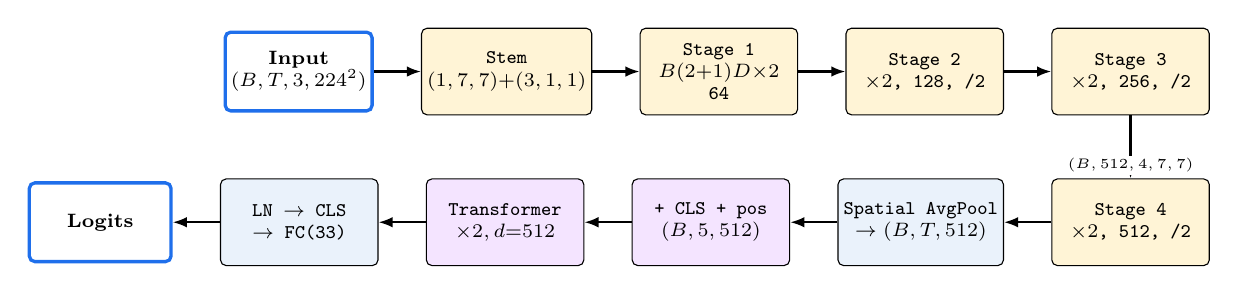
\begin{tikzpicture}[node distance=8mm and 6mm]
    % Row 1 : 3D backbone
    \node[blkio]                          (in)   {Input\\$(B,T,3,224^2)$};
    \node[blkconv, right=of in]           (stem) {Stem\\$(1,7,7){+}(3,1,1)$};
    \node[blkconv, right=of stem]         (s1)   {Stage 1\\$B(2{+}1)D{\times}2$\\64};
    \node[blkconv, right=of s1]           (s2)   {Stage 2\\$\times 2$, 128, /2};
    \node[blkconv, right=of s2]           (s3)   {Stage 3\\$\times 2$, 256, /2};
    % Row 2 : finishing + transformer
    \node[blkconv, below=of s3]           (s4)   {Stage 4\\$\times 2$, 512, /2};
    \node[blkmisc, left=of s4]            (pool) {Spatial AvgPool\\$\to (B,T,512)$};
    \node[blktrans, left=of pool]         (tok)  {+ CLS + pos\\$(B,5,512)$};
    \node[blktrans, left=of tok]          (tx)   {Transformer\\$\times 2, d{=}512$};
    \node[blkmisc, left=of tx]            (head) {LN $\to$ CLS\\$\to$ FC(33)};
    \node[blkio,   left=of head]          (out)  {Logits};

    \draw[flow] (in)--(stem);
    \draw[flow] (stem)--(s1);
    \draw[flow] (s1)--(s2);
    \draw[flow] (s2)--(s3);
    \draw[flow] (s3)--(s4);
    \draw[flow] (s4)--(pool);
    \draw[flow] (pool)--(tok);
    \draw[flow] (tok)--(tx);
    \draw[flow] (tx)--(head);
    \draw[flow] (head)--(out);

    \node[dimlbl, above=1pt of s4] {$(B,512,4,7,7)$};
  \end{tikzpicture}

  \medskip
  \footnotesize
  \textbf{Limites observées.}
  \begin{itemize}
    \item Spatial AvgPool après stage 4 \alert{jette à nouveau} l'information localisée.
    \item L'attention temporelle voit toujours 5 tokens (CLS + 4 frames).
    \item $\Rightarrow$ \hl{flatten plutôt qu'avg-pooler} : c'est model5\_B.
  \end{itemize}
\end{frame}

% =============================================================================
\section{model5\_B : le meilleur from-scratch}
% =============================================================================

\begin{frame}{model5\_B --- 3 changements ciblés vs model5\_A}
  \begin{enumerate}
    \item \hl{Flatten spatio-temporel} après stage 4 : $4 \times 7 \times 7 = \mathbf{196}$ tokens.
    \item \hl{TSM} (Temporal Shift Module) dans chaque BasicBlock : décale $1/8$ des canaux de $\pm 1$ en $T$, \alert{zéro paramètre}.
    \item \hl{Attention pooling} (vecteur query appris) à la place du CLS.
  \end{enumerate}

  \medskip
  \centering
  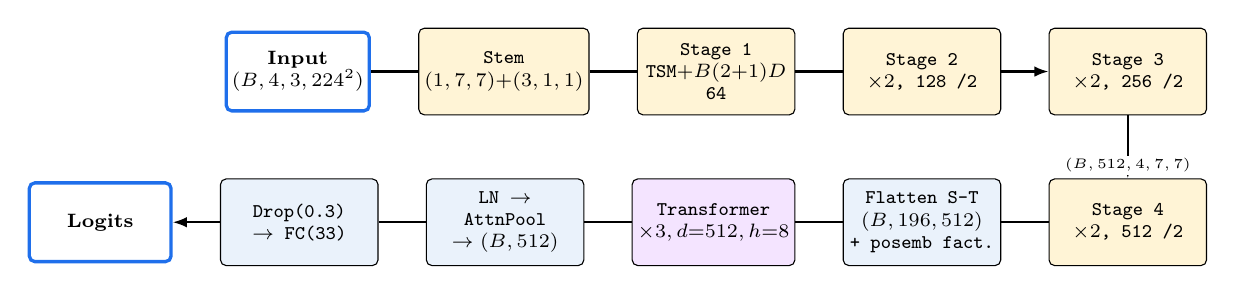
\begin{tikzpicture}[node distance=8mm and 6mm]
    \node[blkio]                          (in)   {Input\\$(B,4,3,224^2)$};
    \node[blkconv, right=of in]           (stem) {Stem\\$(1,7,7){+}(3,1,1)$};
    \node[blkconv, right=of stem]         (s1)   {Stage 1\\TSM$+B(2{+}1)D$\\64};
    \node[blkconv, right=of s1]           (s2)   {Stage 2\\$\times 2$, 128 /2};
    \node[blkconv, right=of s2]           (s3)   {Stage 3\\$\times 2$, 256 /2};

    \node[blkconv,  below=of s3]          (s4)   {Stage 4\\$\times 2$, 512 /2};
    \node[blkmisc,  left=of s4]           (flat) {Flatten S-T\\$(B,196,512)$\\+ posemb fact.};
    \node[blktrans, left=of flat]         (tx)   {Transformer\\$\times 3, d{=}512, h{=}8$};
    \node[blkmisc,  left=of tx]           (ap)   {LN $\to$\\AttnPool\\$\to (B,512)$};
    \node[blkmisc,  left=of ap]           (head) {Drop(0.3)\\$\to$ FC(33)};
    \node[blkio,    left=of head]         (out)  {Logits};

    \draw[flow] (in)--(stem)--(s1)--(s2)--(s3);
    \draw[flow] (s3)--(s4);
    \draw[flow] (s4)--(flat)--(tx)--(ap)--(head)--(out);

    \node[dimlbl, above=1pt of s4] {$(B,512,4,7,7)$};
  \end{tikzpicture}

  \medskip
  \footnotesize \textbf{\good{39.78M params}}, 4.17 ms/clip A100, FP32, single-clip forward.
\end{frame}

\begin{frame}{model5\_B --- entraînement (run v6\_12, best)}
  \begin{columns}[T,onlytextwidth]
    \begin{column}{0.55\textwidth}
      \textbf{Recette d'entraînement.}
      \begin{itemize}
        \footnotesize
        \item AdamW, lr $2\!\cdot\!10^{-5}$, cosine
        \item batch 32 (single GPU)
        \item grad clip 1.0, AMP bf16
        \item MixUp $\alpha{=}0.3$, CutMix $\alpha{=}0.5$ (prob 0.2 / 0)
        \item LS 0.1, dropout3D 0.3, transformer drop 0.2
        \item DropPath 0.1 backbone, 0.3 transformer
        \item Backbone init : \texttt{best\_model\_v3\_36.pt} (R(2+1)D pretrained sur le challenge)
        \item Freeze backbone 5 epochs, puis unfreeze
        \item 80 epochs ($\sim$6 h sur A100)
      \end{itemize}
    \end{column}
    \begin{column}{0.42\textwidth}
      \textbf{Résultats (re-évalués sur le \emph{vrai} val).}
      \begin{center}
        \begin{tabular}{l c}
          \toprule
          Métrique & Valeur \\
          \midrule
          Params totaux       & \good{39.78\,M} \\
          REAL val top-1      & \good{0.406} \\
          REAL val top-5      & \good{0.719} \\
          Latence forward     & 4.17\,ms/clip \\
          Empreinte ckpt      & 159\,MB \\
          \bottomrule
        \end{tabular}
      \end{center}

      \medskip
      \footnotesize
      Meilleur modèle \emph{from scratch} (i.e.\ sans pretrain externe). Le pretrain MAE n'apporte qu'\hl{+0.3\,pts} (cf.\ model7\_A) pour 2,2$\times$ plus de paramètres.
    \end{column}
  \end{columns}
\end{frame}

\begin{frame}{model5\_B --- runs comparés (REAL val top-1)}
  \centering
  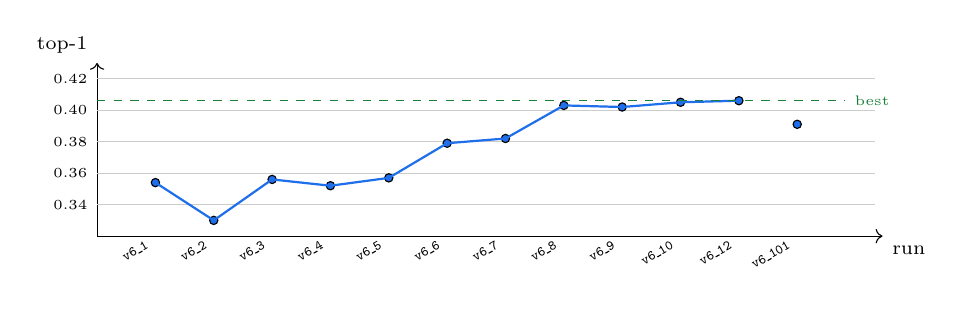
\begin{tikzpicture}[x=0.95cm, y=20cm]
    \draw[->] (0,0.32) -- (10.5, 0.32) node[below right, font=\scriptsize] {run};
    \draw[->] (0,0.32) -- (0, 0.43) node[above left, font=\scriptsize] {top-1};
    \foreach \y in {0.34, 0.36, 0.38, 0.40, 0.42} {
      \draw[gridgray, very thin] (0,\y) -- (10.4,\y);
      \node[left, font=\tiny] at (0,\y) {\y};
    }
    \foreach \i/\yc/\lab in {%
      1/0.354/v6\_1, 2/0.330/v6\_2, 3/0.356/v6\_3, 4/0.352/v6\_4,
      5/0.357/v6\_5, 6/0.379/v6\_6, 7/0.382/v6\_7, 8/0.403/v6\_8,
      9/0.402/v6\_9, 10/0.405/v6\_10, 11/0.406/v6\_12, 12/0.391/v6\_101%
    } {
      \pgfmathsetmacro\xc{\i*0.78}
      \filldraw[fill=accent, draw=black] (\xc, \yc) circle (1.5pt);
      \node[below, font=\tiny, rotate=30, anchor=east] at (\xc, 0.318) {\texttt{\lab}};
    }
    \draw[accent, thick] (0.78, 0.354)
      -- (1.56,0.330) -- (2.34,0.356) -- (3.12,0.352) -- (3.90,0.357)
      -- (4.68,0.379) -- (5.46,0.382) -- (6.24,0.403) -- (7.02,0.402)
      -- (7.80,0.405) -- (8.58,0.406);
    \draw[good, dashed] (0,0.406) -- (10,0.406) node[right, font=\tiny, good] {best};
  \end{tikzpicture}

  \footnotesize Sauts visibles : \texttt{v6\_5$\to$v6\_6} (correction du bug \emph{fake val}) ; \texttt{v6\_7$\to$v6\_8} (DDP 2 GPU, batch effectif 32).
\end{frame}

% =============================================================================
\section{VideoMAE V2 : pretrain self-supervisé}
% =============================================================================

\begin{frame}{VideoMAE V2 --- pretrain self-supervisé}
  \textbf{Objectif.} Apprendre des features vidéo génériques en \alert{reconstruisant les pixels masqués} d'un tubelet. Aucune étiquette.

  \medskip
  \centering
  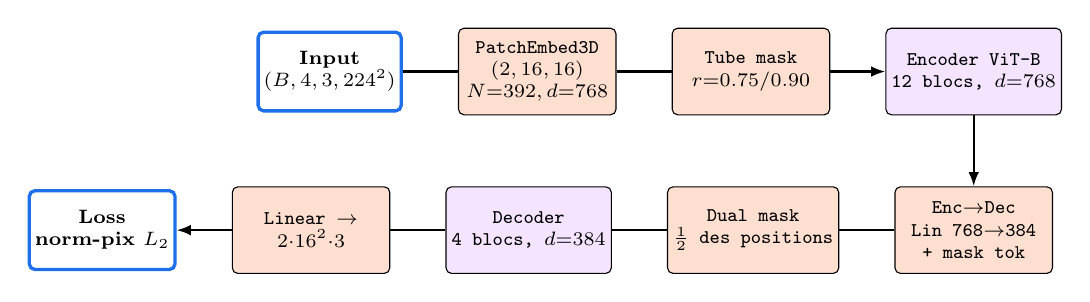
\begin{tikzpicture}[node distance=9mm and 7mm]
    % Row 1 : input -> encoder
    \node[blkio]                          (in)   {Input\\$(B,4,3,224^2)$};
    \node[blkmae,  right=of in]           (pe)   {PatchEmbed3D\\$(2,16,16)$\\$N{=}392, d{=}768$};
    \node[blkmae,  right=of pe]           (tm)   {Tube mask\\$r{=}0.75/0.90$};
    \node[blktrans, right=of tm]          (enc)  {Encoder ViT-B\\12 blocs, $d{=}768$};

    % Row 2 : decoder side, right -> left
    \node[blkmae,   below=of enc]         (proj) {Enc$\to$Dec\\Lin 768$\to$384\\+ mask tok};
    \node[blkmae,   left=of proj]         (dm)   {Dual mask\\$\frac12$ des positions};
    \node[blktrans, left=of dm]           (dec)  {Decoder\\4 blocs, $d{=}384$};
    \node[blkmae,   left=of dec]          (rec)  {Linear $\to$\\$2{\cdot}16^2{\cdot}3$};
    \node[blkio,    left=of rec]          (px)   {Loss\\norm-pix $L_2$};

    \draw[flow] (in)--(pe)--(tm)--(enc);
    \draw[flow] (enc)--(proj);
    \draw[flow] (proj)--(dm)--(dec)--(rec)--(px);
  \end{tikzpicture}

  \medskip
  \footnotesize
  \begin{tabular}{l r r l c}
    \toprule
    Ckpt & mask & epochs & lr & loss finale (recon) \\
    \midrule
    \texttt{mae\_70.pt}        & 0.75 & 196 & 1.5e-4 & \good{0.304} \\
    \texttt{mae\_mask09\_v2.pt} & 0.90 & 200+ & 1e-4 & 0.320 \\
    \bottomrule
  \end{tabular}
\end{frame}

\begin{frame}{Pretrain --- courbes de loss (W\&B)}
  \centering
  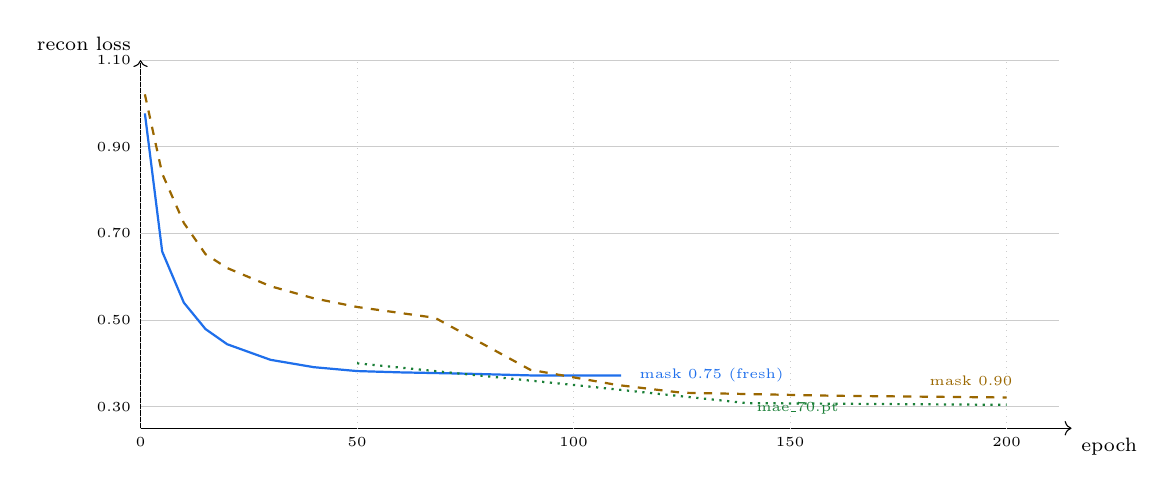
\begin{tikzpicture}[x=0.055cm, y=5.5cm]
    \draw[->] (0, 0.25) -- (215, 0.25) node[below right, font=\scriptsize] {epoch};
    \draw[->] (0, 0.25) -- (0, 1.10) node[above left, font=\scriptsize] {recon loss};
    \foreach \y in {0.30, 0.50, 0.70, 0.90, 1.10} {
      \draw[gridgray, very thin] (0,\y) -- (212,\y);
      \node[left, font=\tiny] at (0,\y) {\y};
    }
    \foreach \x in {0, 50, 100, 150, 200} {
      \draw[gridgray, very thin, dotted] (\x, 0.25) -- (\x, 1.10);
      \node[below, font=\tiny] at (\x, 0.25) {\x};
    }

    % --- mask 0.75 fresh (run iqlvv5j8): 111 epochs, sampled ---
    \draw[accent, thick]
      (1,0.977) -- (5,0.658) -- (10,0.540) -- (15,0.479) -- (20,0.444)
      -- (30,0.408) -- (40,0.391) -- (50,0.382) -- (60,0.379)
      -- (75,0.376) -- (90,0.372) -- (111,0.372);
    \node[accent, font=\tiny, anchor=west] at (113, 0.372) {mask 0.75 (fresh)};

    % --- mask 0.90 (cumulé v2 + part2 + part3): 1->200 ep, sampled ---
    \draw[warn, thick, dashed]
      (1,1.021) -- (5,0.838) -- (10,0.724) -- (15,0.652) -- (20,0.620)
      -- (30,0.578) -- (40,0.550) -- (50,0.530) -- (68,0.505)
      -- (90,0.385) -- (110,0.350) -- (125,0.332) -- (160,0.325) -- (200,0.321);
    \node[warn, font=\tiny, anchor=west] at (180, 0.36) {mask 0.90};

    % --- mask 0.75 orig (sovku5rx) shown only as final 0.304 baseline -- already used
    \draw[good, thick, dotted]
      (50,0.40) -- (100,0.350) -- (140,0.308) -- (200,0.304);
    \node[good, font=\tiny, anchor=west] at (140, 0.295) {mae\_70.pt};
  \end{tikzpicture}

  \footnotesize
  Données extraites des logs W\&B \texttt{iqlvv5j8} (mask 0.75 fresh), \texttt{4ygd8w3y+ap3hg81c+jx29uvim} (mask 0.90 cumulé), \texttt{sovku5rx} (mae\_70).
  \texttt{mask=0.90} ralentit la convergence (\alert{tâche plus dure}) mais converge in fine plus bas.
\end{frame}

% =============================================================================
\section{model7\_A : ViT-B finetune}
% =============================================================================

\begin{frame}{model7\_A --- finetune de l'encoder MAE pour classification}
  \textbf{Idée.} Archi rigoureusement identique à l'encoder MAE $\to$ \texttt{load\_from\_videomae\_v2()} recopie 100\,\% du backbone.

  \medskip
  \centering
  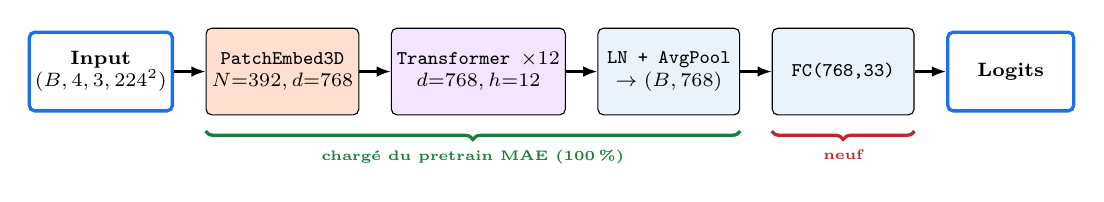
\begin{tikzpicture}[node distance=5mm and 4mm,
                      blkconv/.append style={minimum width=18mm},
                      blktrans/.append style={minimum width=22mm},
                      blkmae/.append style={minimum width=18mm},
                      blkmisc/.append style={minimum width=18mm},
                      blkio/.append style={minimum width=16mm}]
    \node[blkio]                       (in)     {Input\\$(B,4,3,224^2)$};
    \node[blkmae,  right=of in]        (pe)     {PatchEmbed3D\\$N{=}392, d{=}768$};
    \node[blktrans, right=of pe]       (blocks) {Transformer $\times 12$\\$d{=}768, h{=}12$};
    \node[blkmisc, right=of blocks]    (ln)     {LN + AvgPool\\$\to (B,768)$};
    \node[blkmisc, right=of ln]        (fc)     {FC(768,33)};
    \node[blkio,   right=of fc]        (out)    {Logits};

    \draw[flow] (in)--(pe);
    \draw[flow] (pe)--(blocks);
    \draw[flow] (blocks)--(ln);
    \draw[flow] (ln)--(fc);
    \draw[flow] (fc)--(out);

    % Braces below
    \draw[good, very thick, decoration={brace, mirror, amplitude=3pt}, decorate]
      ($(pe.south west)+(0,-2mm)$) -- ($(ln.south east)+(0,-2mm)$)
      node[midway, below=3pt, font=\tiny\bfseries, good]
      {chargé du pretrain MAE (100\,\%)};
    \draw[bad, very thick, decoration={brace, mirror, amplitude=3pt}, decorate]
      ($(fc.south west)+(0,-2mm)$) -- ($(fc.south east)+(0,-2mm)$)
      node[midway, below=3pt, font=\tiny\bfseries, bad]
      {neuf};
  \end{tikzpicture}

  \vspace{4mm}
  \begin{columns}
    \begin{column}{0.5\textwidth}
      \footnotesize
      \textbf{Layer-wise LR decay (LLDR).}
      \[ \text{lr}(\ell) = \text{lr}_{\text{base}} \cdot \gamma^{(D+1-\ell)},\quad \gamma=0.75 \]
      \begin{itemize}
        \item head : full LR
        \item block 11 : $\times 0.75$
        \item patch\_embed : $\times 0.75^{13} \approx 1/24$
        \item $\Rightarrow$ couches basses quasi-gelées
      \end{itemize}
    \end{column}
    \begin{column}{0.5\textwidth}
      \footnotesize
      \textbf{Recette MAE-textbook.}
      \begin{itemize}
        \item AdamW, $\beta_2{=}0.95$, wd 0.05
        \item lr base head $2\!\cdot\!10^{-4}$, warmup 5 ep, cosine $\to 10^{-6}$
        \item MixUp 0.8, CutMix 1.0 (prob 0.5/0.5)
        \item LS 0.1, DropPath 0.2
        \item 50 epochs, batch 24, 86.3M params
      \end{itemize}
    \end{column}
  \end{columns}
\end{frame}

\begin{frame}{Finetune --- LLDR ou pas LLDR ? (W\&B, REAL val top-1)}
  \centering
  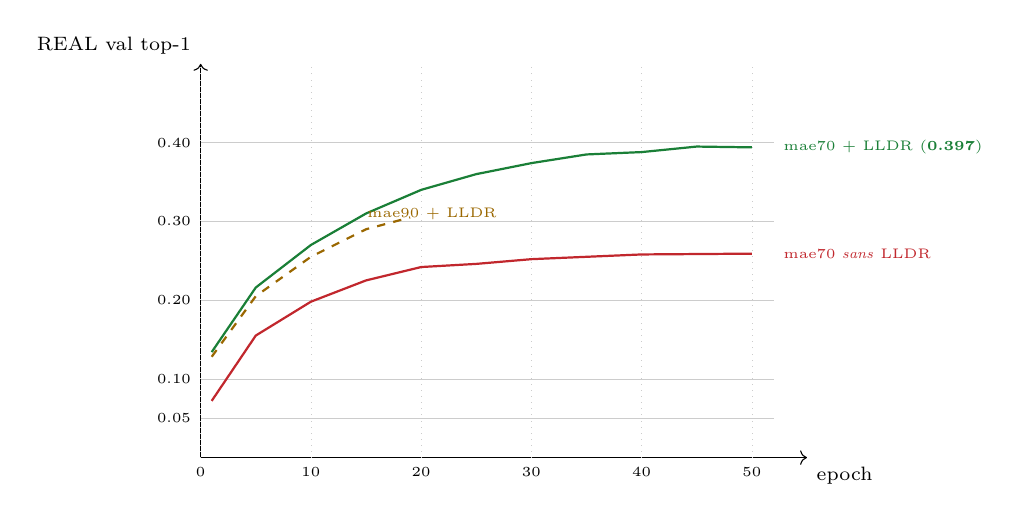
\begin{tikzpicture}[x=0.14cm, y=10cm]
    \draw[->] (0,0) -- (55,0) node[below right, font=\scriptsize] {epoch};
    \draw[->] (0,0) -- (0,0.50) node[above left, font=\scriptsize] {REAL val top-1};
    \foreach \y in {0.05, 0.10, 0.20, 0.30, 0.40} {
      \draw[gridgray, very thin] (0,\y) -- (52,\y);
      \node[left, font=\tiny] at (0,\y) {\y};
    }
    \foreach \x in {0, 10, 20, 30, 40, 50} {
      \draw[gridgray, very thin, dotted] (\x, 0) -- (\x, 0.50);
      \node[below, font=\tiny] at (\x, 0) {\x};
    }

    % ft_mae70_NO_lldr : 50 ep, end 0.2595
    \draw[bad, thick]
      (1,0.072) -- (5,0.155) -- (10,0.198) -- (15,0.225)
      -- (20,0.242) -- (25,0.246) -- (30,0.252) -- (40,0.258) -- (50,0.259);
    \node[bad, font=\tiny, anchor=west] at (52,0.259) {mae70 \emph{sans} LLDR};

    % ft_mae70_lldr_v2 : 50 ep, peaks 0.397 at ep47
    \draw[good, thick]
      (1,0.134) -- (5,0.216) -- (10,0.270) -- (15,0.310)
      -- (20,0.340) -- (25,0.360) -- (30,0.374)
      -- (35,0.385) -- (40,0.388) -- (45,0.395) -- (50,0.394);
    \node[good, font=\tiny, anchor=west] at (52,0.395) {mae70 + LLDR (\good{0.397})};

    % ft_mae90_lldr : 19 ep, end 0.305
    \draw[warn, thick, dashed]
      (1,0.128) -- (5,0.205) -- (10,0.255) -- (15,0.290) -- (19,0.305);
    \node[warn, font=\tiny] at (21,0.31) {mae90 + LLDR};
  \end{tikzpicture}

  \footnotesize
  \alert{Sans LLDR, l'init ViT-B se fait détruire} (head trop forte qui « écrase » les features pretrain) : on ne dépasse pas 0.26 même après 50 epochs.\\
  Avec LLDR sur la même init \texttt{mae\_70.pt}, on atteint \good{0.397} à l'epoch 47.
\end{frame}

\begin{frame}{Finetune --- init mae70 vs mae90 vs mae90 finetune long}
  \centering
  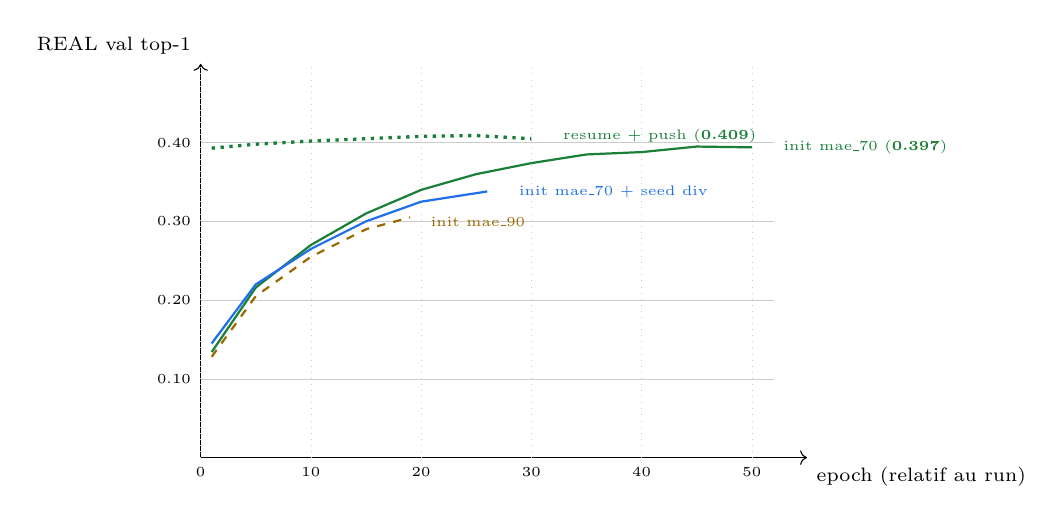
\begin{tikzpicture}[x=0.14cm, y=10cm]
    \draw[->] (0,0) -- (55,0) node[below right, font=\scriptsize] {epoch (relatif au run)};
    \draw[->] (0,0) -- (0,0.50) node[above left, font=\scriptsize] {REAL val top-1};
    \foreach \y in {0.10, 0.20, 0.30, 0.40} {
      \draw[gridgray, very thin] (0,\y) -- (52,\y);
      \node[left, font=\tiny] at (0,\y) {\y};
    }
    \foreach \x in {0, 10, 20, 30, 40, 50} {
      \draw[gridgray, very thin, dotted] (\x, 0) -- (\x, 0.50);
      \node[below, font=\tiny] at (\x, 0) {\x};
    }

    % ft_mae70_lldr_v2 : 50 ep, best 0.397
    \draw[good, thick]
      (1,0.134) -- (5,0.216) -- (10,0.270) -- (15,0.310)
      -- (20,0.340) -- (25,0.360) -- (30,0.374)
      -- (35,0.385) -- (40,0.388) -- (45,0.395) -- (50,0.394);
    \node[good, font=\tiny, anchor=west] at (52, 0.394) {init mae\_70 (\good{0.397})};

    % ft_mae70_diverse seed=100 : 26 ep, end 0.338
    \draw[accent, thick]
      (1,0.145) -- (5,0.220) -- (10,0.265) -- (15,0.300) -- (20,0.325) -- (26,0.338);
    \node[accent, font=\tiny, anchor=west] at (28, 0.338) {init mae\_70 + seed div};

    % ft_mae90_lldr (mae_mask09_v2): 19 ep, 0.305
    \draw[warn, thick, dashed]
      (1,0.128) -- (5,0.205) -- (10,0.255) -- (15,0.290) -- (19,0.305);
    \node[warn, font=\tiny, anchor=west] at (20, 0.30) {init mae\_90};

    % resume diverse from lldr_v2 + push : final 0.409
    \draw[good, very thick, dotted]
      (1,0.393) -- (5,0.398) -- (10,0.402) -- (15,0.405) -- (20,0.408) -- (25,0.409) -- (30,0.405);
    \node[good, font=\tiny, anchor=west] at (32, 0.409) {resume + push (\good{0.409})};
  \end{tikzpicture}

  \footnotesize
  Toutes courbes extraites de W\&B (\texttt{zan03dr2}, \texttt{pndm6gsf}, \texttt{2if09wfz}, \texttt{gpxf7uzm}).
  \hl{mae\_70 (mask=0.75) bat mae\_90} en finetune ; le run final \good{lldr\_diverse} reprend \texttt{lldr\_v2} et le pousse à 0.409 grâce à un resume + augs diversifiées.
\end{frame}

% =============================================================================
\section{Bilan}
% =============================================================================

\begin{frame}{Coût d'entraînement vs accuracy}
  \centering
  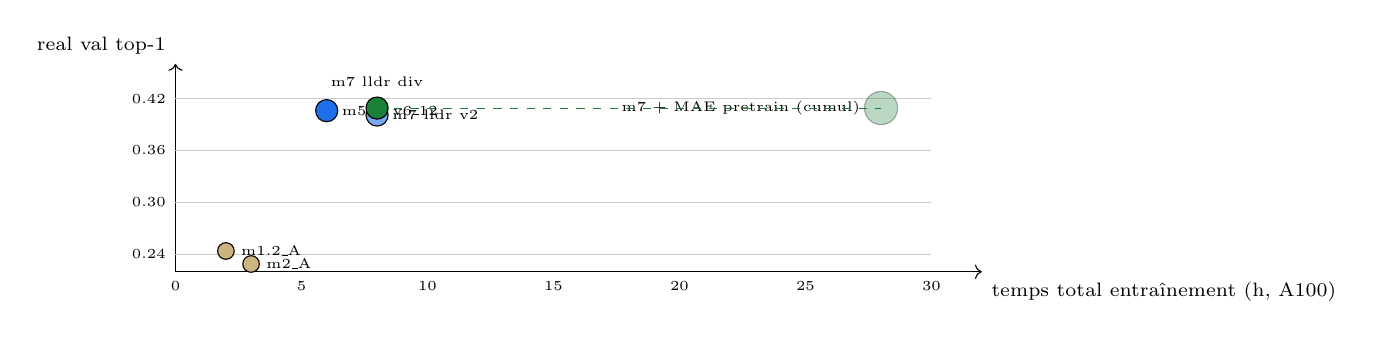
\begin{tikzpicture}[x=0.32cm, y=11cm]
    \draw[->] (0, 0.22) -- (32, 0.22) node[below right, font=\scriptsize] {temps total entraînement (h, A100)};
    \draw[->] (0, 0.22) -- (0, 0.46) node[above left, font=\scriptsize] {real val top-1};
    \foreach \y in {0.24, 0.30, 0.36, 0.42} {
      \draw[gridgray, very thin] (0,\y) -- (30, \y);
      \node[left, font=\tiny] at (0, \y) {\y};
    }
    \foreach \x in {0, 5, 10, 15, 20, 25, 30} {
      \node[below, font=\tiny] at (\x, 0.22) {\x};
    }
    \filldraw[fill=warn!50] (2, 0.244) circle (3pt);
    \node[right=2pt, font=\tiny] at (2,0.244) {m1.2\_A};
    \filldraw[fill=warn!50] (3, 0.229) circle (3pt);
    \node[right=2pt, font=\tiny] at (3,0.229) {m2\_A};
    \filldraw[fill=accent] (6, 0.406) circle (4pt);
    \node[right=2pt, font=\tiny] at (6,0.406) {m5\_B v6\_12};
    \filldraw[fill=accent!60] (8, 0.401) circle (4pt);
    \node[right=2pt, font=\tiny] at (8,0.401) {m7 lldr v2};
    \filldraw[fill=good] (8, 0.409) circle (4pt);
    \node[above=3pt, font=\tiny] at (8,0.413) {m7 lldr div};
    \filldraw[fill=good, opacity=0.3] (28, 0.409) circle (6pt);
    \node[left=4pt, font=\tiny] at (28, 0.409) {m7 + MAE pretrain (cumul)};
    \draw[good, dashed] (8, 0.409) -- (28, 0.409);
  \end{tikzpicture}

  \footnotesize
  \begin{itemize}\setlength{\itemsep}{1pt}
    \item Le \alert{vrai coût} de \texttt{model7\_A} inclut le pretrain MAE ($\sim$22\,h pour \texttt{mae\_70}).
    \item En coût total, \texttt{model5\_B} est \hl{$\sim$5$\times$ plus efficace} pour 0.3\,pts de moins.
  \end{itemize}
\end{frame}

\begin{frame}{Ce qui ressort de ces expériences}
  \begin{columns}[T,onlytextwidth]
    \begin{column}{0.5\textwidth}
      \good{Ce qui paie}
      \begin{itemize}
        \item \hl{Prior 3D} (R(2+1)D) >> attention 2D pure.
        \item \hl{TSM} : gratuit, indispensable avec $T{=}4$.
        \item \hl{Plus de tokens} (196 vs 5) : laisse l'attention exister.
        \item \hl{Attention pooling} > CLS pour grand $N$.
        \item \hl{LLDR} \emph{indispensable} pour finetuner un ViT pretrainé MAE.
        \item \hl{Vrai val} pour sélectionner le checkpoint.
      \end{itemize}
    \end{column}
    \begin{column}{0.48\textwidth}
      \alert{Ce qui n'a pas marché}
      \begin{itemize}
        \item Pretrain MAE court ($\leq 200$ ep) : ViT-B reste limite vs R(2+1)D 40M.
        \item \texttt{mask\_ratio=0.90} : finetune moins bon ($-7$\,pts vs mask 0.75).
        \item Empiler dropout / drop\_path sans aug données : plafonne.
        \item Run \texttt{fresh\_500} : warm-restart mal configuré ($\to 0.027$).
        \item Finetune \emph{sans} LLDR : plafonne à 0.26.
      \end{itemize}
    \end{column}
  \end{columns}
\end{frame}

\begin{frame}
  \begin{center}
    \Large \textbf{Meilleur modèle} \\[0.5em]
    \texttt{model7\_lldr\_diverse} : ViT-B finetune depuis MAE\\
    86.3\,M params, top-1 \good{0.409}, top-5 \good{0.736} \\[0.6em]
    \emph{Mais} : \texttt{model5\_B v6\_12} suit à 0.3\,pts, avec \good{39.8\,M} params seulement.
  \end{center}
\end{frame}

\end{document}
